\chapter{How to Use MATSim Extensions \who{Zilske}}
\label{ch:extensionpoints}
% ##################################################################################################################
\hfill \textbf{Authors:} Michael Zilske

\kai{M.E.\ ist das hier vor allem die ``script''-Syntax, um die ``contribs'' einzubinden. Eigene Extensions kommen m.E.\ sp�ter, entweder in ``contributing to MATSim'', oder wir nehmen das dort raus.  (Wir wollen ``contributions to MATSim'' doch als Nutzer der extension points, und nicht immer gleich als Leute, die den core anfassen, oder?)}

\kai{Habe den Titel schonmal entsprechend angepasst (war vorher ``how to extend MATSim'').}

\ah{Evtl. w�rde ich dann doch daf�r pl�dieren ``contributing to MATSim'' nach hier vorne zu verschieben. Damit w�re dann klar: MATSim wird nur an den Extensions-Points ``penetriert''. Bin mittlerweile �berzeugt, dass Core-Anfassen im Buch gar nicht vorkommen sollte ... andere Leserschaft.}

\begin{center} 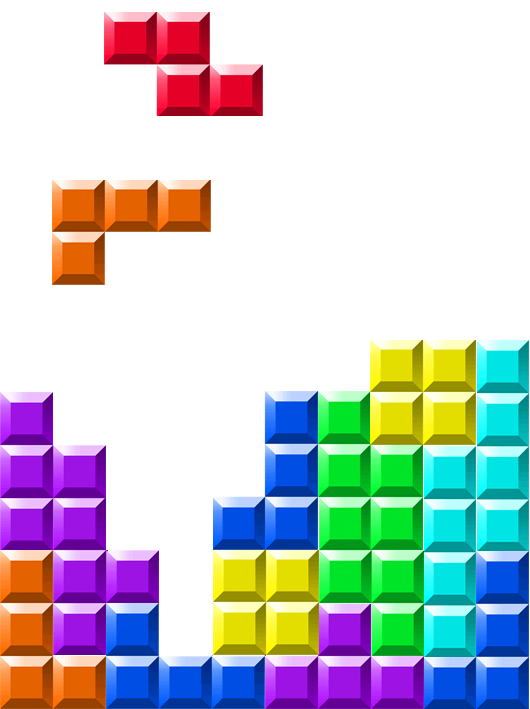
\includegraphics[width=0.25\textwidth, angle=0]{figures/MATSimBook.png} \end{center}

% ##################################################################################################################
MATSim Extension Points

auch etwas MATSim-Architecture


% ##################################################################################################################
\section{Events}
\label{sec:events}

% ##################################################################################################################
\section{Listener Architecture}

% ##################################################################################################################
\section{Personalized Controler}



% ##################################################################################################################
